\begin{frame}{GATr - Introduzione}
    In diverse situazioni si ha a che fare con dati di natura geometrica, soprattutto
    in ambiti scientifici ed ingegneristici. Il vantaggio di utilizzare dati geometrici
    risiede nel comportamento definito dei dati sotto trasformazioni ben definite 
    (come distanze e rotazioni).

    Con l'obiettivo di utilizzare nel modo migliore questi dati, si introduce il 
    Geometric Algebra Transformer (GATr), un'architettura di rete general-purpose 
    che sfrutta dati geometrici. 
\end{frame}

\begin{frame}{GATr - Idee Chiave}
    GATr integra tre concetti fondamentali:
    \begin{itemize}
        \item \textbf{Algebra Geometrica}
        \item \textbf{Equivarianza}
        \item \textbf{Transformer}
    \end{itemize}
\end{frame}

\begin{frame}{Algebra Geometrica}

    Per rappresentare oggetti tridimensionali e applicare rotazioni e traslazioni su di 
    essi, la 3D GA non è sufficiente, poichè i multivettori dell'algebra tradizionale 
    possono rappresentare solo sottospazi lineari che passano per l'origine e rotazioni 
    intorno ad essa. 

    GATr consente di rappresentare i dati come multivettori dell'algebra geometrica 
    proiettiva \(\mathbb{G}_{3,0,1}\). In pratica lo spazio di interesse viene inserito 
    in uno spazio di dimensione superiore, aggiungendo una quarta coordinata omogenea 
    \(x_0 \Vb{e}_{0}\), ottenendo un'algebra di dimensione \(2^4 = 16\) dimensioni, capace di 
    rappresentare vari tipi geometrici e pose \(E(3)\).
\end{frame}

\begin{frame}{Algebra Geometrica}

    Nell’algebra geometrica, un vettore \( \Vb{u} \) può agire come operatore riflettendo 
    altri elementi nel piano ortogonale a \( \Vb{u} \). 
    Poiché ogni trasformazione ortogonale può essere espressa come una sequenza di riflessioni, 
    possiamo rappresentare qualsiasi trasformazione come prodotto geometrico di vettori 
    unitari, detti \textit{versori}  \( u = u_1 \cdots u_k \).

    Il prodotto di versori unitari genera un gruppo, chiamato \textit{Pin group}, 
    in cui i versori unitari si comportano come propri inversi (\( u^2 = 1 \)). 
    I prodotti di un numero pari di riflessioni formano il \textit{Spin group}. 
    Nell’algebra geometrica proiettiva \( \mathbb{G}_{3,0,1} \), questi gruppi 
    permettono di coprire le trasformazioni \( E(3) \) e \( SE(3) \), rispettivamente.
\end{frame}

\begin{frame}{Algebra Geometrica: Prodotto Sandwich}
    Le simmetrie tridimensionali (rotazioni, traslazioni, riflessioni) si rappresentano 
    con i multivettori di \( \mathbb{G}_{3,0,1} \). Il prodotto \textit{sandwich} applica 
    un versore \( u \) ad un elemento \( x \):

    \[
        \rho_u(x) = 
        \begin{cases}
            u x u^{-1} & \text{se } u \text{ è pari} \\
            u x \hat{u}^{-1} & \text{se } u \text{ è dispari}
        \end{cases}
    \]

    dove \( \hat{x} \) è l'involuzione di grado, che inverte il segno degli elementi 
    dispari (come vettori e trivettori) e lascia invariati quelli di grado pari. 
    Questo prodotto fornisce una rappresentazione lineare dei gruppi \textit{Pin} e 
    \textit{Spin}.

\end{frame}

\begin{frame}{Algebra Geometrica}

    Per rappresentare oggetti 3D, i piani sono descritti da vettori, e l'intersezione 
    di due oggetti geometrici è data dal prodotto wedge delle loro rappresentazioni. 
    Si crea una dualità tra oggetti e operatori, in cui gli oggetti 
    si comportano come trasformazioni che li lasciano invariati.

    La Tabella mostra una corrispondenza tra queste rappresentazioni, che risultano 
    compatibili con il prodotto \textit{sandwich} utilizzato per le trasformazioni.

\end{frame}

\begin{frame}{Algebra Geometrica: Tabella di Oggetti e Operatori}
    \begin{figure}
        \centering
        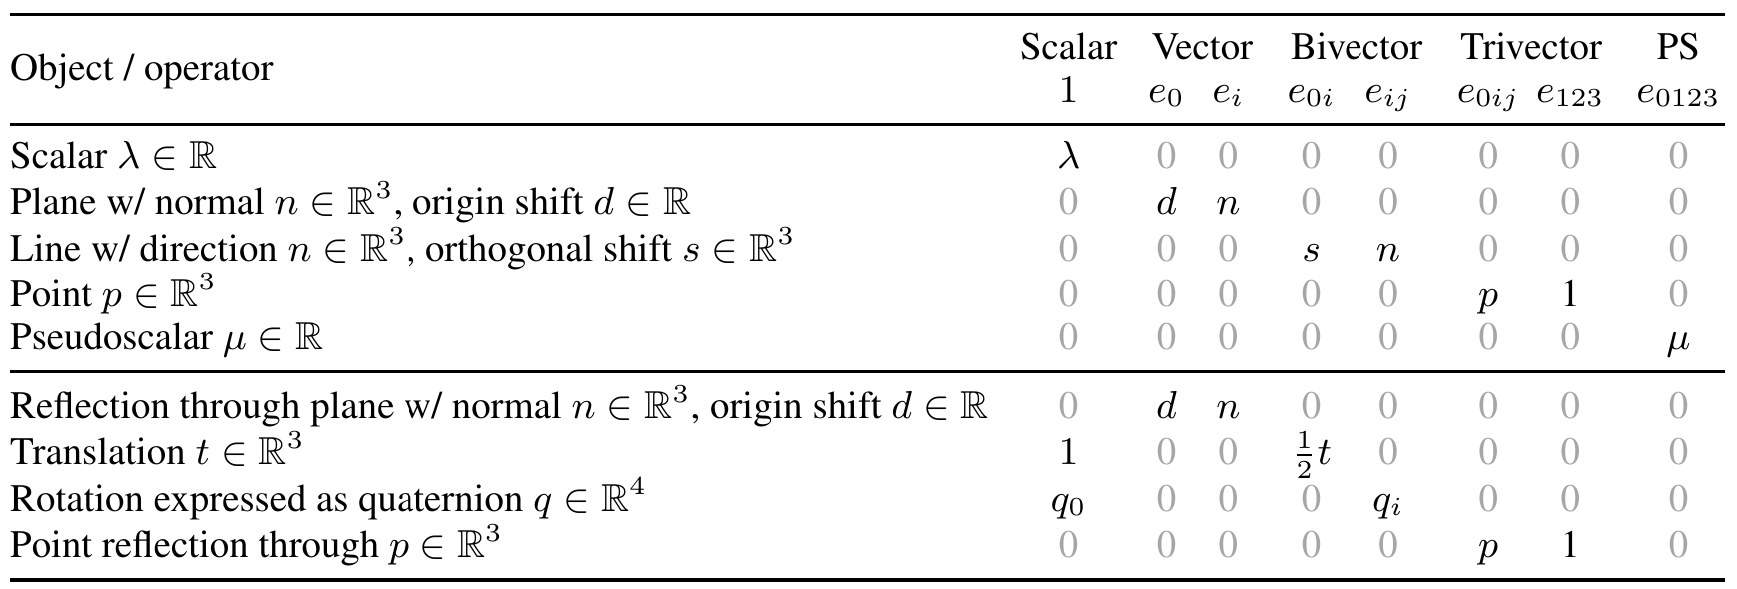
\includegraphics[width=0.9\textwidth]{../Images/relazioneOggettiOperatori.png}
        \caption{Tabella di oggetti 3D e trasformazioni}
    \end{figure}
\end{frame}

\begin{frame}{Equivarianza}
    GATr è progettato per essere equivariante rispetto al gruppo di simmetria \(E(3)\), 
    che descrive le trasformazioni nello spazio tridimensionale. 

    A tale scopo, sono state sviluppate diverse nuove primitive 
    \(E(3)\)-equivarianti, tra cui mappe lineari equivarianti, un meccanismo di 
    attenzione, non-linearità e strati di normalizzazione.

    Vengono costruiti networks layers che sono equivarianti rispetto a \(E(3)\). 
    Una funzione \( f : \mathbb{G}_{3,0,1} \) è \( Pin(3,0,1) \)-equivariante rispetto
    alla rappresentazione \( p \) se 
    \[
        f(p_u(x)) = p_u(f(x))
    \]
    per ogni \( u \in Pin(3,0,1) \) e \(x \in \mathbb{G}_{3,0,1}\), dove \( p_u(x) \) è 
    il sandwich product definito in \eqref{eq:4}
\end{frame}

\begin{frame}{Trasformer}
    Per il GATr si è scelto di utilizzare l'architettura Transformer grazie alle sue 
    favorevoli proprietà di scalabilità, espressività, addestrabilità e versatilità.

    Di seguito si analizza più nel dettagli la struttura di questo modello.
\end{frame}